
以前常常把“evolution”译作“进化”,但“进化”并非都是进步的,现在多把“evolution”称作“演化”。达尔文认为,演化是“有变化的传代”(descent with modification)。

\section{进化理论的百家争鸣}

林奈与布丰是同时代的人,他们的观点相悖:

\begin{itemize}
	\item 林奈是物种不变论的代表人物,认为神创造了多少物种就有多少物种;
	\item 布丰反对物种不变论,但在教会的威胁下屈服。
\end{itemize}

\subsection{拉马克学说的创建过程}

\subsubsection{斗争——居维叶的灾变论}

居维叶(法国)提出了\sy{器官相关定律}:一个动物体内各器官在结构与功能上是相互协调的,一个器官的形态特征可以推断出其他器官的特征,进而推知整个动物的形态与生活方式。

居维叶在研究了不同地层中的化石后,提出灾变论:地球在不同时间、地点发生巨大的灾难,毁灭了当时的生物,之后又有别的生物迁入,因而在不同地层中留下不同的化石。

\subsubsection{拉马克的进化理论}

与居维叶不同,拉马克却认为这些化石是生物进化的证据。

拉马克提出了“环境影响生物体”的学说。内容如下:

\begin{description}
	\item[环境条件的转变引起生物变异] 环境对植物和低等动物的影响是直接的,对高等动物的影响是间接的,需要通过动物的主观行为改变。
	\item[用进废退] 经常使用的器官变得发达,不使用的器官退化。
	\item[获得性状遗传] 器官用或不用导致的变异是可以遗传的。
	\item[等级进化] 生物具有按等级向上发展的趋向。
\end{description}

此外,拉马克还认为最原始的生物是自然发生的,支持生命多起源。现在发现,“获得性状遗传”似乎具有表观遗传学基础。

\subsection{达尔文学说的创立}

\subsubsection{前提——生命科学的进展}

\begin{itemize}
	\item 胡克观察到了活细胞;
	\item 居维叶提出器官相关定律;
	\item 圣提雷尔提出同源器官和同工器官的概念;
	\item 沃尔弗提出胚胎发育的渐成说;
	\item 地层年龄和化石复杂度的关系。
\end{itemize}

进化论的形成是科学发展的必然结果。此外,达尔文本人乘Beagle舰的经历也有很大影响。

\subsubsection{达尔文的理论}

自然选择是渐进的过程。达尔文接受了拉马克的用进废退和获得性状遗传,但自然选择学说与其完全不同。达尔文主张物种可变论和单起源。


\begin{description}
	\item[过度繁殖] 达尔文接受马尔萨斯“人口论”的影响,认为繁殖过剩引起生存斗争。
	\item[生存斗争] 包括种内、种间、与无机环境的斗争。通过生存斗争实现优胜劣汰。
	\item[适应的起源] 达尔文认为,适应是两步适应,即变异+选择=适应。强调变异的不定向性。这与拉马克不同。
\end{description}

赫胥黎是达尔文学说的拥护者,他与教会进行的“牛津大论战”给他赢得了“达尔文的斗士”称号。

达尔文还提出了人工选择学说,即人类按照自己的标准挑选产生变异的个体,导致微小变异的积累,最终形成多个新品种。

\subsection{进化理论的发展}

\subsubsection{现代综合进化论}

也称为现代达尔文主义,代表人物是杜布赞斯基。他完成了对现代综合进化论的综合。

该学说主要内容是:

\begin{itemize}
	\item 自然选择决定进化的方向,主张两步适应;
	\item 种群是进化的基本单位。进化的实质就是种群内基因频率和基因型频率的改变;
	\item 突变、选择、隔离是物种形成和生物演化的机制。结构基因中的点突变为进化提供了原始素材,通过自然选择使群体基因频率定向改变,隔离阻断基因交流;
\end{itemize}

\subsubsection{米丘林学说}

\begin{itemize}
	\item 早年接受拉马克的观点,认为变异是定向的。变异是对环境改变的直接适应;
	\item 后来较多接受了达尔文的观点,在人工选择理论的基础上开展育种研究;
	\item 米丘林学派否认不定向的变异和突变在进化中的作用,认为“如果获得性状不遗传就不存在生物进化”。
\end{itemize}

\subsubsection{分子进化中性论}

主要代表人物是木村资生。

中性突变指的是不影响蛋白质功能的突变,即无害也无利,如同工突变和同义突变。通过漂变导致突变的积累,导致生物形态和生理出现差异,最后通过自然选择产生表形进化。

\subsubsection{近中性理论}


\subsubsection{间断平衡论}

间断平衡论主张进化是突变和渐变交替的。

\subsubsection{新灾变论}

不同于居维叶的灾变论,抛弃了神创论的色彩,主张一个物种在实际上保持不变的时期被突发事件打断,由此从原有种那里产生新的后裔种。

\section{生命的产生}

\subsection{对生命起源的朴素认识}

\subsubsection{自然发生论}

认为生命可以自发从非生命物质中直接迅速产生,如腐草为萤、白石化羊、腐肉生蛆等。

\subsubsection{神创论}

将生命起源归因为超自然力量的干预,并认为物种之间是互不相关、永恒不变的。

\subsubsection{生生论、宇生论}

意大利医生Redi用实验证明腐肉不能生蛆,巴斯德用鹅颈瓶实验彻底否定自然发生论,支持生生论。

宇生论认为生命来自于太空。现在发现地外确实存在有机物,但并不一定表明生命来自地球之外。

\subsubsection{新自然发生论}

德国的奥肯提出最初的生命来源于“原始粘液”,所有的有机物都从这里演化而来。

\subsection{生命起源的化学学说}

\subsubsection{米勒实验}

米勒模拟了早期地球的条件,能源是火花放电,最终合成出Gly、Ala、Asp、Val等氨基酸。(\autoref{fig:miller-ureyexperiment-en})

\begin{figure}[h]
	\centering
	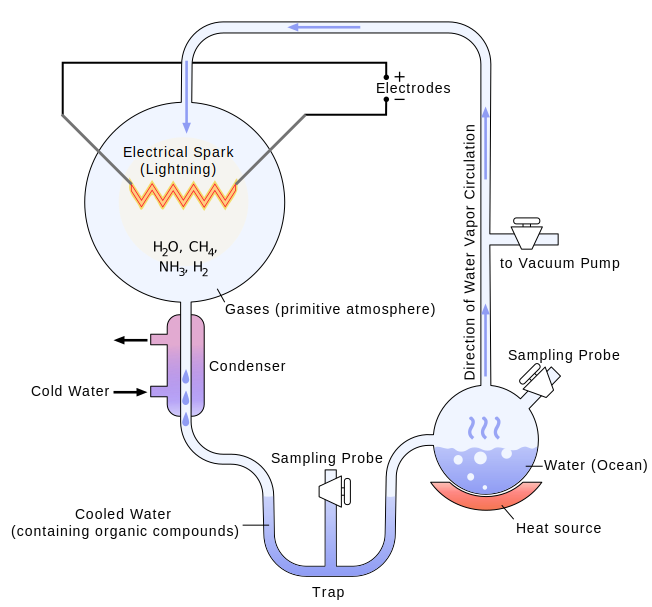
\includegraphics[width=0.7\textwidth]{Miller-Urey_experiment-en}
	\caption{米勒实验}
	\label{fig:miller-ureyexperiment-en}
\end{figure}


\subsubsection{核酸和蛋白质起源先后之争}

多数学者认为核酸和蛋白质同时起源。

\paragraph{起源方式——三大学说}

陆相起源说:福克斯,大陆火山附近。在大陆火山附近的水池里生成大量的氨基酸,在火山喷发时被强烈的高温蒸发干枯,剩下的氨基酸发生热聚合脱水而成高聚物,雨水把高聚物带到原始海洋中,在海水的作用下,高聚物(多肽)经过自我装配形成蛋白质,在火山区形成核酸的过程也与此类似。补充:发现在蛋白质合成过程中,酸性氨基酸的比例加大,则更有利于类蛋白质的合成。

海相起源说:霍洛维茨、卡恰尔斯基,在原始海洋中,相对分子质量小的氨基酸和核苷酸可以被吸附到黏土、蒙脱石一类物质的活性表面,在适当的缩合剂存在时,脱水、缩合成相对分子质量高的聚合物。实验:Gly+ATP的水溶液,加入沸石$\longrightarrow$生成甘氨酰腺嘌呤核苷磷酸$\longrightarrow$在碱性溶液中被吸附到蒙脱石的活性表面,经聚合产生了类蛋白质。

深海“烟囱”起源说:斯坦利,如\autoref{fig:深海烟囱起源说}所示:

\begin{figure}[htb]
	\centering
	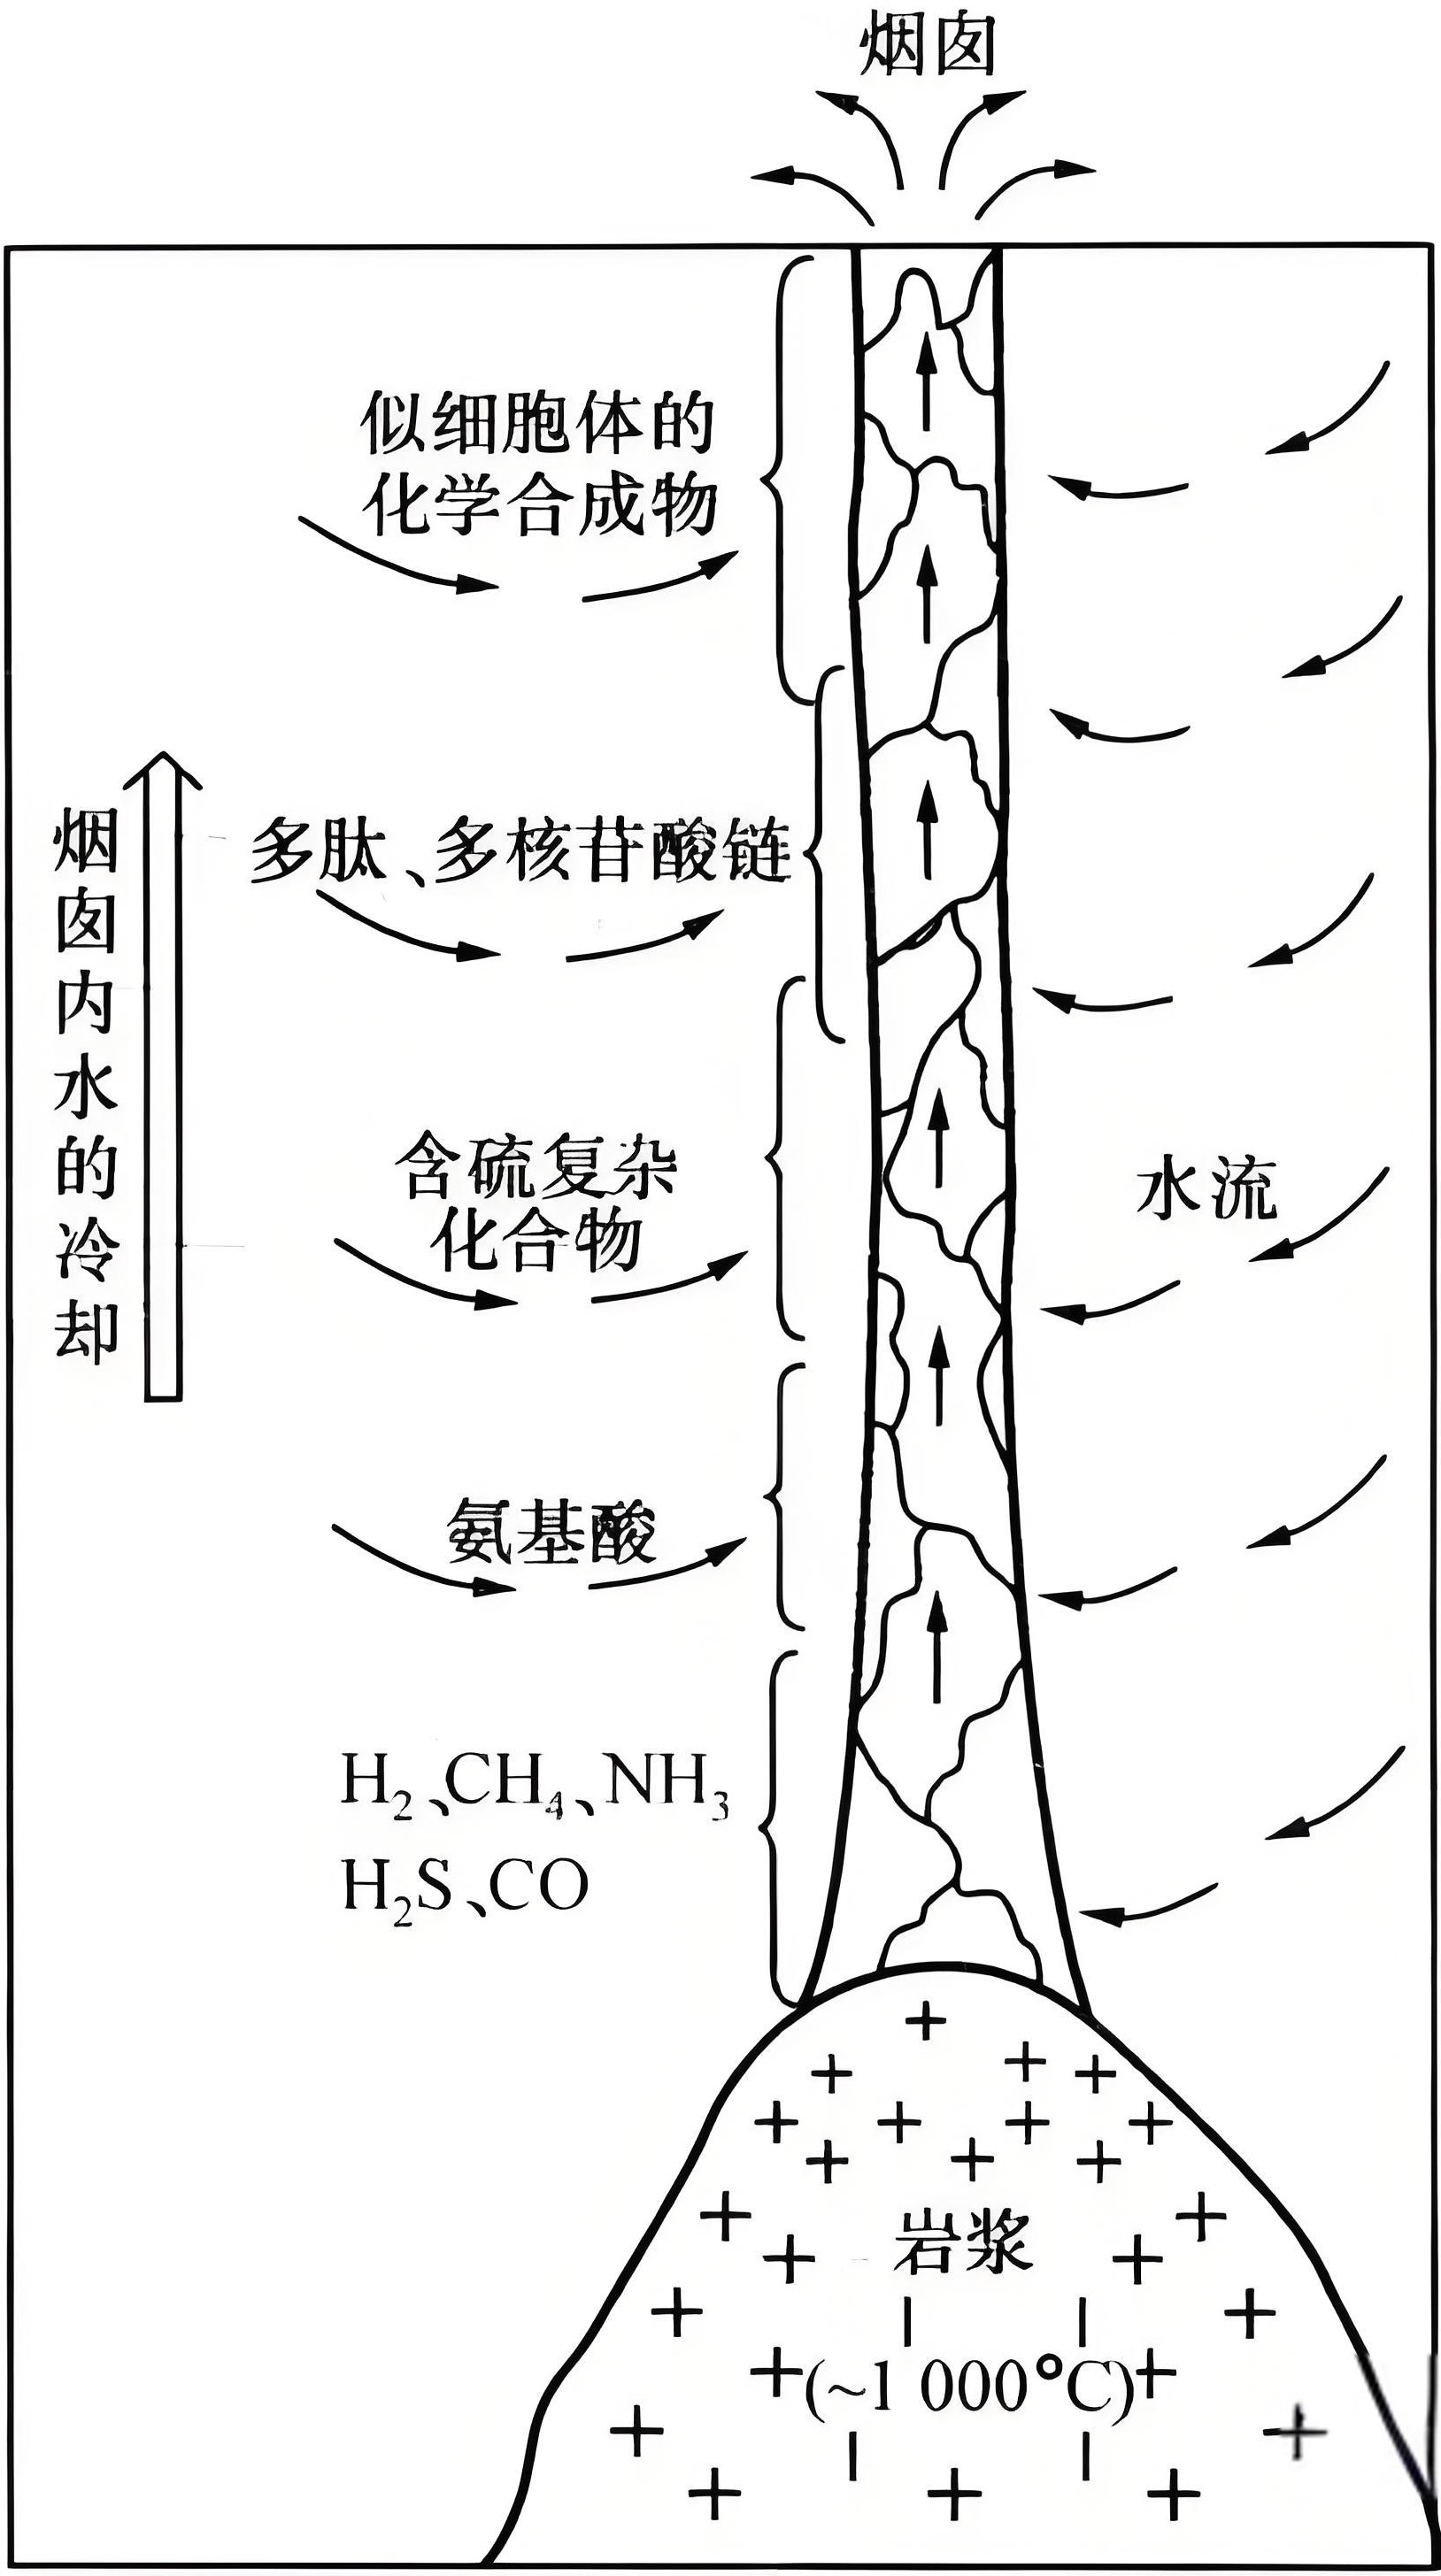
\includegraphics[width=0.4\linewidth]{深海烟囱起源说}
	\caption{深海烟囱起源说}
	\label{fig:深海烟囱起源说}
\end{figure}

\subsection{遗传密码的演化}

Dayhoff通过计算机程序发现:

\begin{itemize}
	\item 不同生物的同一种tRNA是由共同祖先的tRNA分子分支演化而来;同一种生物体内不同种tRNA则没有这种进化关系;
	\item 所有tRNA的祖先分子中,CG含量远远超过AU,随着生物的进化,AU含量逐渐增加,线粒体tRNA的AU含量增加得更加显著。
\end{itemize}

进化顺序:GNC$\longrightarrow$GNY$\longrightarrow$RNY$\longrightarrow$RNN$\longrightarrow$NNN(R代表嘌呤,Y代表嘧啶)

\begin{enumerate}
	\item GNC和GNY阶段:仅第二碱基决定氨基酸种类,实质上相当于单体密码,第一位和第三位决定转译的方向(仅编码G、A、E、V四种氨基酸,恰恰符合米勒实验得到的四种最多的氨基酸);
	\item RNY阶段:由第一和第二碱基决定氨基酸种类,实质上相当于二体密码;
	\item RNN和NNN阶段:三个碱基都不同程度的参与了氨基酸种类的决定,实质上已过渡到真正的三体密码。
	\begin{enumerate}
		\item RNN:第三次扩展,出现起始密码子;
		\item NNN:第四次扩展,出现终止密码子,那些具有复杂侧链的氨基酸对应的密码子也在这一次出现。
	\end{enumerate}
\end{enumerate}

\section{化石和地质年代划分}

\subsection{化石}

按保存特点,可分为:

\begin{description}
	\item[遗体化石] 古生物的遗体形成的化石,如动物的骨骼化石、植物的茎秆化石等。还可细分为变质和不变质的两种。变质的化石即生物成分被矿质取代,一般化石越古老,石化程度越高。不变质的如在冻土中发现的猛犸、琥珀中的昆虫。
	\item[模铸化石] 生物体在基质中留下的印记,分为印痕化石和印模化石。简单来说,印痕化石偏平面,印模化石偏立体。
	\item[遗物化石] 古代动物的粪便、卵,植物的汁液、人类祖先使用的工具等。
	\item[遗迹化石] 古代动物活动时留下的痕迹。如古人类的脚印。
\end{description}

按功能可分为:

\begin{description}
	\item[标准化石] 可用作其所在地质年代标志的化石,因为其存在时间较短。
	\item[指相化石] 能够指示当时地层沉积环境的化石,如贝壳化石指相为水。
	\item[标记物化石] 古代大分子留下的降解产物,如叶绿素降解产物植烷的出现表明光合作用的产生。
\end{description}

\subsection{地质年代的划分}

地质年代的划分见\autoref{tab:earth_age}。

\begin{landscape}
	\begin{table}[h!]
		\zihao{5}
		\centering
		\begin{tabularx}{\linewidth}{|ccccCC|}
			\hline
			\multicolumn{3}{|c|}{\multirow{2}{*}{地层年代}} & \multicolumn{1}{c|}{\multirow{2}{*}{Mya}} & \multicolumn{2}{c|}{生命演化事件} \\ \cline{5-6} 
			\multicolumn{3}{|c|}{} & \multicolumn{1}{c|}{} & \multicolumn{1}{C|}{植物} & 动物 \\ \hline
			\multicolumn{3}{|c|}{冥古宙} & \multicolumn{1}{c|}{4600\textasciitilde 4000} & \multicolumn{2}{c|}{地球形成} \\ \hline
			\multicolumn{3}{|c|}{太古宙} & \multicolumn{1}{c|}{4000\textasciitilde 2500} & \multicolumn{2}{c|}{最早生命形式出现} \\ \hline
			\multicolumn{3}{|c|}{元古宙} & \multicolumn{1}{c|}{2500\textasciitilde 541} & \multicolumn{2}{c|}{蓝细菌产氧,多细胞生物出现} \\ \hline
			\multicolumn{1}{|c|}{\multirow{16}{*}{显生宙}} & \multicolumn{1}{c|}{\multirow{8}{*}{古生代}} & \multicolumn{1}{c|}{寒武纪} & \multicolumn{1}{c|}{541\textasciitilde 485} & \multicolumn{2}{c|}{寒武纪生命大爆发} \\ \cline{3-6} 
			\multicolumn{1}{|c|}{} & \multicolumn{1}{c|}{} & \multicolumn{1}{c|}{奥陶纪} & \multicolumn{1}{c|}{485\textasciitilde 444} & \multicolumn{1}{c|}{藻类繁盛} & 无颌鱼类出现 \\ \cline{3-6} 
			\multicolumn{1}{|c|}{} & \multicolumn{1}{c|}{} & \multicolumn{4}{c|}{大灭绝} \\ \cline{3-6} 
			\multicolumn{1}{|c|}{} & \multicolumn{1}{c|}{} & \multicolumn{1}{c|}{志留纪} & \multicolumn{1}{c|}{444\textasciitilde 419} & \multicolumn{1}{c|}{维管植物登陆} & 有颌鱼类出现 \\ \cline{3-6} 
			\multicolumn{1}{|c|}{} & \multicolumn{1}{c|}{} & \multicolumn{1}{c|}{泥盆纪} & \multicolumn{1}{c|}{419\textasciitilde 359} & \multicolumn{1}{c|}{种子蕨出现} & 两栖、昆虫出现,脊椎登陆 \\ \cline{3-6} 
			\multicolumn{1}{|c|}{} & \multicolumn{1}{c|}{} & \multicolumn{4}{c|}{大灭绝} \\ \cline{3-6} 
			\multicolumn{1}{|c|}{} & \multicolumn{1}{c|}{} & \multicolumn{1}{c|}{石炭纪} & \multicolumn{1}{c|}{359\textasciitilde 299} & \multicolumn{1}{c|}{森林繁盛,煤炭形成} & 爬行出现 \\ \cline{3-6} 
			\multicolumn{1}{|c|}{} & \multicolumn{1}{c|}{} & \multicolumn{1}{c|}{二叠纪} & \multicolumn{1}{c|}{299\textasciitilde 252} & \multicolumn{1}{c|}{松柏出现} & 爬行繁盛 \\ \cline{2-6} 
			\multicolumn{1}{|c|}{} & \multicolumn{1}{c|}{\multirow{5}{*}{中生代}} & \multicolumn{1}{c|}{三叠纪} & \multicolumn{1}{c|}{252\textasciitilde 201} & \multicolumn{1}{c|}{苏铁、银杏出现} & 恐龙出现 \\ \cline{3-6} 
			\multicolumn{1}{|c|}{} & \multicolumn{1}{c|}{} & \multicolumn{4}{c|}{大灭绝} \\ \cline{3-6} 
			\multicolumn{1}{|c|}{} & \multicolumn{1}{c|}{} & \multicolumn{1}{c|}{侏罗纪} & \multicolumn{1}{c|}{201\textasciitilde 145} & \multicolumn{1}{c|}{被子植物出现} & 恐龙繁盛 \\ \cline{3-6} 
			\multicolumn{1}{|c|}{} & \multicolumn{1}{c|}{} & \multicolumn{1}{c|}{白垩纪} & \multicolumn{1}{c|}{145\textasciitilde 66} & \multicolumn{1}{c|}{被子植物繁盛} & 胎盘类、现代昆虫出现 \\ \cline{3-6} 
			\multicolumn{1}{|c|}{} & \multicolumn{1}{c|}{} & \multicolumn{4}{c|}{大灭绝} \\ \cline{2-6} 
			\multicolumn{1}{|c|}{} & \multicolumn{1}{c|}{\multirow{3}{*}{新生代}} & \multicolumn{1}{c|}{古近纪} & \multicolumn{1}{c|}{66\textasciitilde 23} & \multicolumn{1}{c|}{被子植物演化} & 哺乳类演化 \\ \cline{3-6} 
			\multicolumn{1}{|c|}{} & \multicolumn{1}{c|}{} & \multicolumn{1}{c|}{新近纪} & \multicolumn{1}{c|}{23\textasciitilde 2.6} & \multicolumn{1}{c|}{草本植物广布} & 人类祖先出现 \\ \cline{3-6} 
			\multicolumn{1}{|c|}{} & \multicolumn{1}{c|}{} & \multicolumn{1}{c|}{第四纪} & \multicolumn{1}{c|}{2.6\textasciitilde \hspace{-0.12em}现在} & \multicolumn{2}{c|}{人类破坏} \\ \hline
		\end{tabularx}
		\caption{地质年代表}
		\label{tab:earth_age}
	\end{table}
\end{landscape}

\section[哈-温平衡及其拓展]{哈迪-温伯格平衡及其拓展}

\subsection[基本的哈-温平衡]{基本的哈迪-温伯格平衡}

\subsubsection{哈迪-温伯格平衡的概念}

在一定条件下,种群内基因频率和基因型频率保持不变,就属于\sy{哈迪-温伯格平衡}。需要满足的条件有:无突变、无选择、无迁移、随机交配、种群足够大。

\zhongdian{哈迪-温伯格平衡实际上是一种理想情况,现实中不可能有种群满足上述全部条件。}

\subsubsection{用数学表达哈迪-温伯格平衡}

设种群中一对等位基因\textit{A}、\textit{a}的基因频率分别为$p, q$,基因型频率\textit{AA}、\textit{Aa}、\textit{aa}分别为$D=p^{2}, H=2pq, R=q^{2}$。

可以知道,群体平衡$\Leftrightarrow H=2\sqrt{DR}$。

当两性染色体连锁基因频率不等时,雌性基因频率$p_{f}, q_{f}$和雄性基因频率$p_{m}, q_{m}$在一代随机交配后,有如下关系:



\subsubsection{选择、突变对平衡的影响}

在下面的叙述中,约定

\paragraph{选择对隐性纯合子不利}

假设完全显性,将\textit{AA}和\textit{Aa}个体适合度记为1,\textit{aa}个体适合度为$s$,则\textit{a}基因频率改变量\[\upDelta q=\frac{-sq^{2}(1-q)}{1-sq^{2}}\approx-sq^{2}(1-sq)\]


推导如下:

设初始项为 \(s_0\),递推关系为\[s_n = \frac{s_{n-1}}{1 + s_{n-1}}, \quad n \ge 1.\]取倒数,令\[t_n = \frac{1}{s_n}.\]
则
\[t_n 
= \frac{1 + s_{n-1}}{s_{n-1}}
= \frac{1}{s_{n-1}} + 1
= t_{n-1} + 1.
\]
由此得到
\[
t_n = t_0 + n
\quad\Longrightarrow\quad
\frac{1}{s_n} = \frac{1}{s_0} + n.
\]
反写得
\[
s_n 
= \frac{1}{\dfrac{1}{s_0} + n}
= \frac{s_0}{1 + n\,s_0}.
\]
若序列从 \(n=1\) 开始,且 \(s_1 = a\),则同理
\[
\frac{1}{s_n} = \frac{1}{s_1} + (n-1) = \frac{1}{a} + (n-1),
\]
因此
\[
s_n 
= \frac{1}{\dfrac{1}{a} + (n-1)}
= \frac{a}{1 + (n-1)\,a}.
\]



